\subsection{The transverse slope estimate}

The exact calculation is now summarized by
Lemma~\ref{lem:hko-exact-bounds}. We use only its rank and positivity
statements in the remaining argument.

\begin{lemma}[Uniformly negative transverse slopes]\label{lem:hko-negative-slopes}
Choose a linear complement $S$ to the symmetry tangent space $T$, so that
$(\mathbb R^4)^{10}=T\oplus S$ and $\dim S=25$.
There is $\eta>0$ such that
\[
 \min_{1\leq j\leq26}r_j(v)\leq-\eta\|v\|
 \qquad\text{for every }v\in S.
\]
\end{lemma}
\begin{proof}
The rows have rank twenty-five and vanish on the fifteen-dimensional
space $T$. Their common kernel is therefore exactly $T$, and their
restrictions span $S^*$.
For $v\in S\setminus\{0\}$, suppose that every $r_j(v)$ were
nonnegative. Their positively weighted sum is zero, so each would have
to vanish. Then $v\in T\cap S=\{0\}$, a contradiction.
Thus $\min_jr_j(v)<0$ for every nonzero transverse direction.

The function $v\mapsto\min_jr_j(v)$ is continuous on the unit sphere of
$S$. Its maximum there is strictly negative by compactness. Write that
maximum as $-\eta$ and use homogeneity to obtain the assertion.
\end{proof}

Figure~\ref{fig:hko-upper-mechanism} illustrates the slope condition in
one and two transverse dimensions.
\begin{figure}[htbp]
\centering
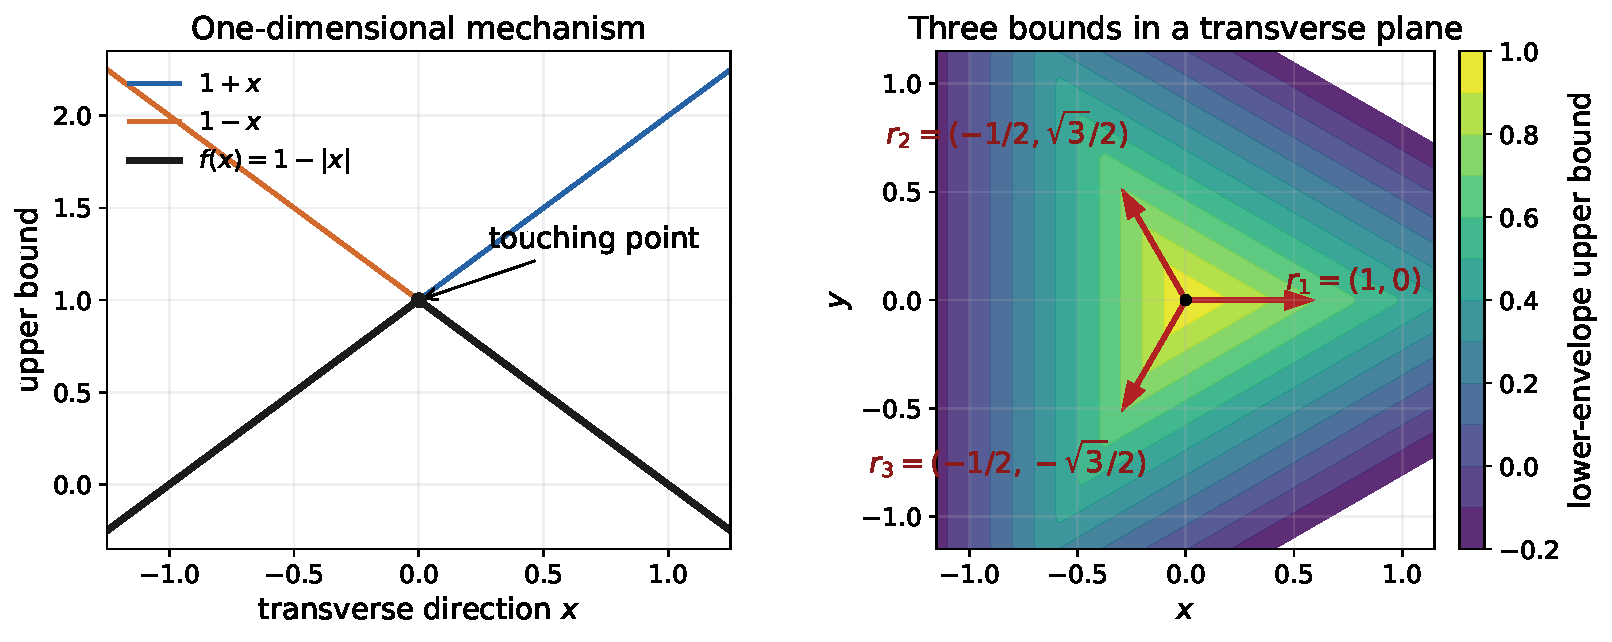
\includegraphics[width=\linewidth]{recovered/hko-figures/upper-bound-mechanisms.pdf}
\caption{Toy models of touching upper bounds. Left: the lower envelope of
$1+x$ and $1-x$ is $1-|x|$. Right: level sets of the lower envelope of
three affine functions with gradients
$(1,0)$, $(-1/2,\sqrt3/2)$ and $(-1/2,-\sqrt3/2)$.
The gradients span the plane and sum to zero, and the envelope decreases
in every nonzero direction. In the proof the systolic ratio lies below
the envelope and agrees with it at the base point.}
\label{fig:hko-upper-mechanism}
\end{figure}

\subsection{From slopes to a neighborhood}

We now pass from the derivative estimate to nearby bodies. The uniform
constant $\eta$ lets us choose one neighborhood for all transverse
directions.

\begin{lemma}[Strict decrease on the slice]\label{lem:hko-slice-decrease}
For all sufficiently small nonzero $v\in S$,
\[
 \operatorname{sys}(K(a_0+v))
 \leq\operatorname{sys}(K_0)-\frac\eta2\|v\|
 <\operatorname{sys}(K_0).
\]
\end{lemma}
\begin{proof}
There are only twenty-six smooth upper bounds. Their differentiability
at $a_0$ therefore supplies a common neighborhood in which
\[
 |U_j(a_0+v)-U_j(a_0)-r_j(v)|
 \leq\frac\eta2\|v\|\qquad(j=1,\ldots,26).
\]
Shrink it so that all bounds are defined and dominate the ratio there.
For each $v\in S$, Lemma~\ref{lem:hko-negative-slopes} supplies an index
with $r_j(v)\leq-\eta\|v\|$. Since $U_j(a_0)=\operatorname{sys}(K_0)$,
\[
 \operatorname{sys}(K(a_0+v))\leq U_j(a_0+v)
 \leq\operatorname{sys}(K_0)-\frac\eta2\|v\|.\qedhere
\]
\end{proof}

\begin{lemma}[Local symmetry decomposition]\label{lem:hko-symmetry-decomposition}
Every row list sufficiently close to $a_0$ is the image of some
$a_0+v$, with $v\in S$ small, under a symmetry close to the identity.
The symmetry and $v$ can be chosen smoothly in local group coordinates.
\end{lemma}
\begin{proof}
Translation by $y$, dilation by $\rho>0$ and a linear symplectic map $M$
act on the rows, respectively, by
\[
 a_i\mapsto\frac{a_i}{1+a_i\cdot y},\qquad
 a_i\mapsto\rho^{-1}a_i,\qquad
 a_i\mapsto M^{-T}a_i.
\]
These actions are smooth near the identity. Choose fifteen local
coordinates $\theta$ for this symmetry group and write its action as
$g(\theta)$. The map
\[
 \Phi(\theta,v)=g(\theta)\cdot(a_0+v),\qquad v\in S,
\]
has derivative at $(0,0)$ with image $T$ in the group variables and
image $S$ in the slice variables. The fifteen symmetry derivatives are
independent by Lemma~\ref{lem:hko-exact-bounds}. Thus $D\Phi(0,0)$ is
an isomorphism, and the inverse function theorem gives the decomposition.
\end{proof}

The toy model in Figure~\ref{fig:hko-symmetry-extension} shows how a
strict transverse maximum becomes a family of equal maxima along symmetry.
\begin{figure}[htbp]
\centering
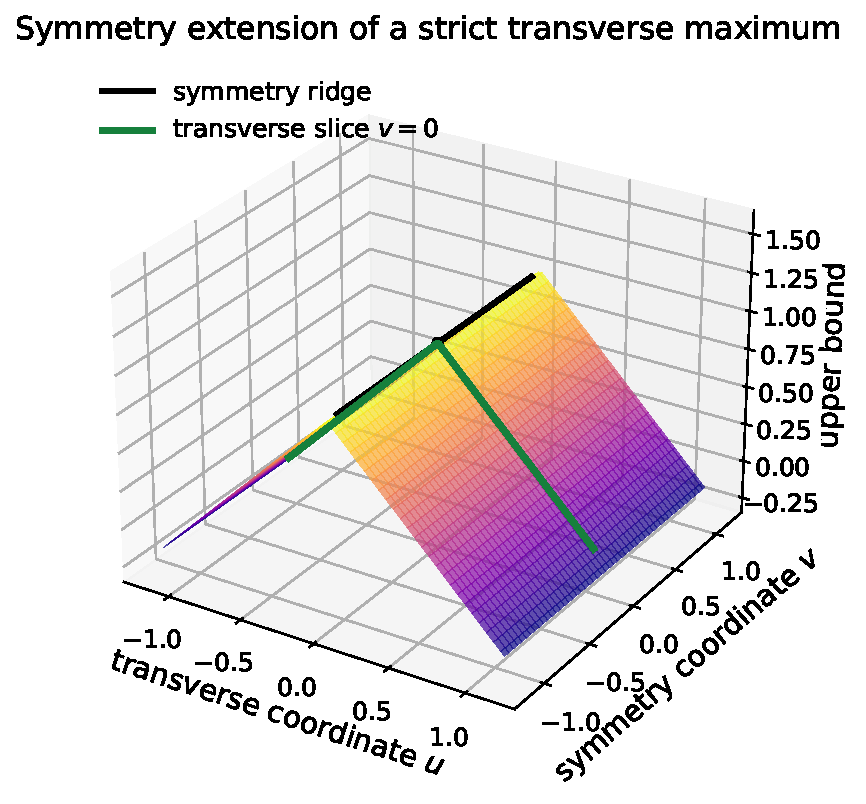
\includegraphics[width=0.72\linewidth]{recovered/hko-figures/symmetry-extension.pdf}
\caption{The toy function $f(u,v)=1-|u|$ has a strict maximum on the
transverse slice $v=0$ and is constant along the symmetry coordinate $v$.
Its maxima form the ridge $u=0$. In the HKO proof the symmetry tangent
space $T$ has dimension fifteen and the transverse space $S$ has dimension
twenty-five. The picture illustrates their roles in the local decomposition.}
\label{fig:hko-symmetry-extension}
\end{figure}

\begin{proof}[Proof of Theorem~\ref{thm:hko-ten-facet-local-maximum}]
By Lemma~\ref{lem:hko-row-neighborhood}, a sufficiently Hausdorff-close
ten-facet body has a row list in the neighborhood of
Lemma~\ref{lem:hko-symmetry-decomposition}. It is therefore a symmetry
image of $K(a_0+v)$ for some small $v\in S$. The ratio is unchanged by
that symmetry. Lemma~\ref{lem:hko-slice-decrease} gives a strict decrease
if $v\ne0$, and equality if $v=0$. Equality consequently forces the
body to be a symmetry image of $K_0$. Conversely, every such image
has the same ratio as $K_0$.
\end{proof}
